\documentclass[12pt,oneside,a4paper]{article} 
\usepackage[utf8]{inputenc}
\usepackage{graphicx}
\usepackage{subcaption}
\usepackage[T1]{fontenc}
\usepackage{parskip}
\usepackage{tabularx}
\usepackage{booktabs}
\usepackage{listings}
\usepackage{color}
\usepackage{pifont}
\usepackage{setspace}
\usepackage{tikz}
\usepackage{todonotes}
\usepackage{mathptmx}
\usepackage{setspace}
\usepackage{titlesec}
\usepackage[top=2cm, bottom=2cm, left=3cm, right=3cm]{geometry}
\usepackage[hidelinks]{hyperref}

\lstset{
    % frame=single, 
    language=sql, 
    basicstyle=\footnotesize,
    numbers=left, 
    numberstyle=\tiny\color{darkgray}, 
    keywordstyle=\color{blue}, 
    commentstyle=\color{gray},
    otherkeywords={IF, SCHEMA, USE, REFERENCES, AUTO_INCREMENT, DATETIME}
}

\pagestyle{plain}

\newcommand{\HRule}{\rule{\linewidth}{0.5mm}}

\begin{document}
	\begin{titlepage}
    \begin{center}
        
        % Upper part of the page. The '~' is needed because \\
        % only works if a paragraph has started.
        
        \textsc{\Large Database Systems \\
            02170 \\ 
            Fall 2015 \\ 
            DTU Compute \\ 
            Technical University of Denmark}\\[1.5cm]
        
        %\textsc{\Large Project Group 8}\\[0.5cm]
        
        % Title
        \HRule \\[0.4cm]
        { \huge \bfseries Train Management \\[0.4cm] }
        
        \HRule \\[1.5cm]
        
        % Author and supervisor
        \begin{center}
            \begin{minipage}{0.5\textwidth}
                \begin{flushleft} \large
                    \emph{Authors:}\\
                    Christoffer \textsc{Hjort} \\
                    s144224 \\ ~\\
                    Tobias Skovlund \textsc{Petersen} \\
                    s123302
                \end{flushleft}
            \end{minipage}
        \end{center}
        
        \vfill
        
        % Bottom of the page
        {\large \today}
        
    \end{center}
\end{titlepage}
    \setcounter{page}{2}
	\tableofcontents
	
	\section{Introduction}
% Christoffer

% Introduction to train management:
The database system of this project is a train management schema, which stores trains, stations, tracks, routes, employees, etc. So a railway system that connects cities and stations is what we are modelling with our 'Train Management' scheme.\\
This report will go through process of designing the database system, implementing it, the programming, and using it.\\[12pt]
The functionality of this databse system is to store important stuff about a railway system, like routes and tracks between cities and stations. With the relations in this 'Train Management' scheme it is possible to plan a route from, for example, station A to station B and calculate the shortest route to reach the destination.\\ However, these more advanced algorithms, \textit{"Breadth-first search"} and \textit{"Dijkstra's Shortest Path"}, to plan routes and calculate shortest paths, are not implemented or stored as procedures in this schema, as they are tough to implement with our current SQL programming knowledge.
The 'Train Management' schema is however compatible with the implementation of these algorithm. So by using the correct queries on the relations it is definitely possible to retrieve the required information that these algorithms need, and they could then be implemented in another DBMS like ODBC or JDBC.\\[12pt]
Database type*
% What is the purpose? 
	%Describe part of real world to be modelled
% What is this report about?
% What functionality do we want?
	%Be able to have cities and stations be connected by routes and tracks, and store it in our database?
	%Be able to plan routes?
% What are the limitations, i.e. is there something we are not goint to include?
	%Complicated graph algorithms to calculate 		shortest routes etc. are not implemented
	%Could have used BFS and Dijkstra's to make a routeplanning stored procedure.

% What sort of database is it? 
% (Production, Transaction, Fulltext, Temporal or Data Warehouse database)
	\section{Design} \label{sec:design}

This section describes the requirements of the database, and how the Entity 
Relation diagram was designed to facilitate those requirements. 

\subsection{Requirements}

We want our database to be compatible for storing train systems and planning 
routes. Therefore we want parts of our database relations to easily resemble 
graph structures. These ``graph'' relations are specifically \emph{Station}, 
\emph{Route}, \emph{Track}, and \emph{RouteTracks}.

That is, \emph{Station} can be seen as the relation containing vertices, and 
\emph{Track} containing the edges between vertices. \emph{RouteTracks} then 
contains a composition of tracks/edges to resemble a route that connects 
through different stations/vertices.

The other relations like \emph{Train}, \emph{Employees} and \emph{Shift} are 
not really key parts of our database functionality, but are relations that 
should be included none the less.

As general description of our desired database is as follows:
The train management system i organized into stations. Stations have a number 
of lanes, and are located in cities. Stations are connected to each other with 
tracks. A track therefore always have a station in each of its endpoints and 
has a given length. Routes have a start and stop station. A route is composed 
of multiple tracks, and spans over several stations. The length of a route 
should be possible to calculate from its tracks contained.

A train can ride on an existing route. There is no limit for the amount of trains driving at the same time. A train has a model, production year and an age. An employee can have a work shift on a train, and the shift has a start time and end time. An employee has unique initials, a name, and an address.

\subsection{Functionality}
% Functional requirements:
% Views:
%  * Length of a route
%  * View stations on a route
% Functions / Triggers / ... Mention functionality of those (NOT how they were 
% implemented)
There are certain functionalities that we want our \emph{Train Management} 
schema to have, and these functionalities are what should define our schema as 
being a database for managing train systems and planning routes.

These functionalities are accomplished with the use of views, functions, 
triggers, procedures, etc.

Some of the most essential functionalities we want our database to have is
\begin{itemize}
\item Be able to find the length of a route.
\item Be able to find the stations on a route.
\item Data integrity
\item Compatibility for depth search algorithms and shortest routes algorithms.
\end{itemize}

Fortunately, simple views can be used to easily find the length of a route and its stations. These views are describes in the implementation section. So is a trigger that helps with data integrity of station lanes, by preventing illegal inserts. The compatibility for applying graph algorithms is achieved with the design of our relations, shown on the ER diagram below.

\subsection{ER diagram}
Figure~\ref{fig:ER} shows our ER diagram, which illustrates the design of our 
\emph{Train Management} schema. It shows that some entities have total 
participation in some of the relations, as for instance you can not have tracks 
without stations or cities, neither can you have routes without tracks.

\begin{figure}[ht!]
    \centering
    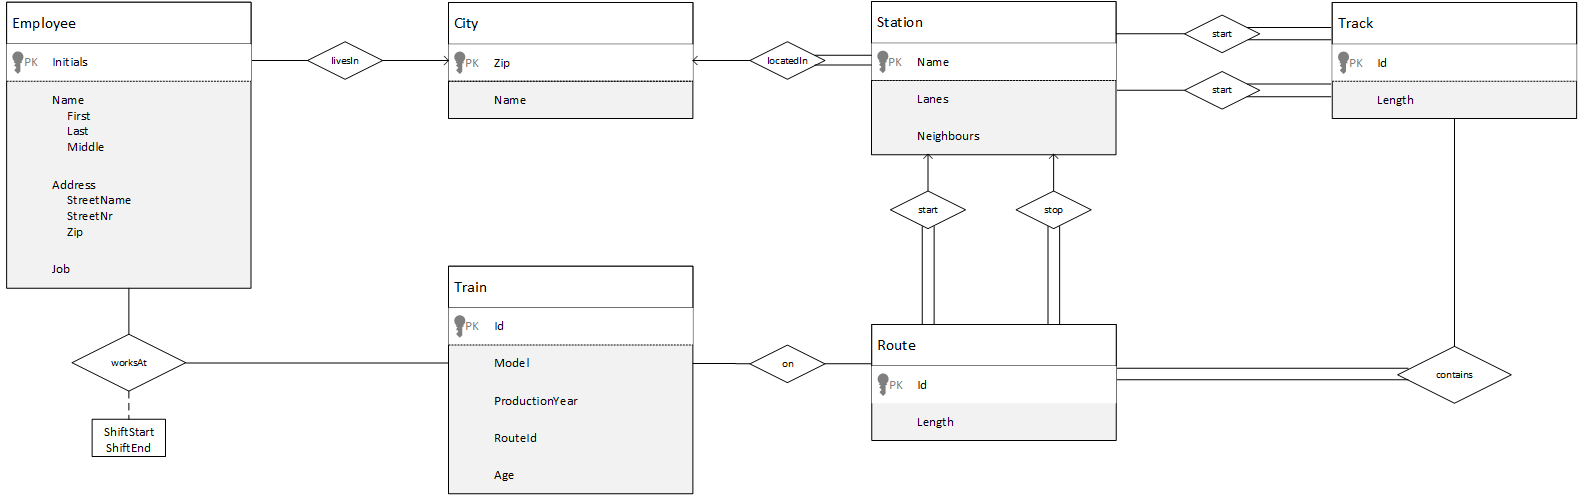
\includegraphics[angle=90,origin=c,width=.45\textwidth]{img/Handwritten_ER}
    \caption{An ER diagram depiction the design of the database}
    \label{fig:ER}
\end{figure}

% Design coices 
% See notes on hand drawn ER diagram (marked by *) None of those 3 examples 
% have been mentioned

% Comments on ER diagram supporting the requirements
The relations \emph{Station} and \emph{Track} are purposely designed to resemble "graph" relations as described in the requirements. This enables the possible implementation of graph-algorithms, with \emph{Stations} being nodes/vertices and \emph{Track} as edges.
\\[12pt]
Further functionalities and advancements could have been done in the form of including timestamps and time as a general factor for route-planning etc. Due to the scale of the project and keeping it realistically achievable at the same time, it has been decided to not include time in any form, other than the workshift start and end times.\\
The ER diagram shows total participation between \emph{Route} and 
\emph{RouteTracks}. This however is really tricky to have implemented in the 
SQL Schema. In fact it is not implemented in the current schema. This is 
discussed in the implementation section.

	\section{Implementation}

% Forward / Backward engineering

% 


\subsection{MySQL EER Diagram}



\subsection{Functionality} % Other title?

% Specs require: Functions, procedures, transactions, triggers and events
% Make sure to include all of these in the design or possibly in the intro

    \section{Database programming}\label{sec:prog}
This section deals with populating the database, updating and deleting existing 
entries, and finally some SQL programming.

\subsection{SQL Data Manipulation}
When inserting into the empty schema, it is necessary to insert cities as the 
first thing. Next is stations, followed by tracks, routes, trains, employees, 
etc. This is because of the relations and their total participation in each 
other. For example, a track can not exist without having a station in each 
end.
Also, when inserting data into a relation, the values of the insert statement 
of course has to correspond with the relation design on our ER diagram.\\
An example of inserting cities, would be done by statements like the following:

\begin{figure}[ht!]
    \centering
    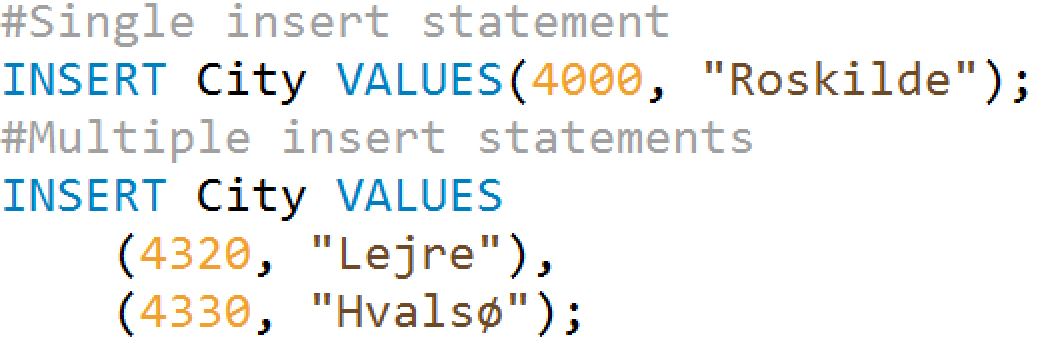
\includegraphics[width=.6\textwidth]{img/INSERT_Statements}
    \caption{SQL INSERT statements for City}
\end{figure}

It is now possible to insert stations located in the existing cities

\begin{figure}[ht!]
    \centering
    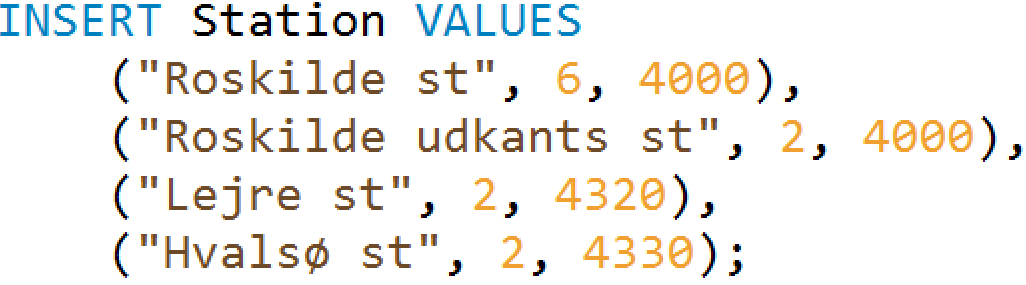
\includegraphics[width=1\textwidth]{img/INSERT_Statement_Station}
    \caption{SQL INSERT statements for Station}
\end{figure}

and then connect these stations with tracks.

\begin{figure}[ht!]
    \centering
    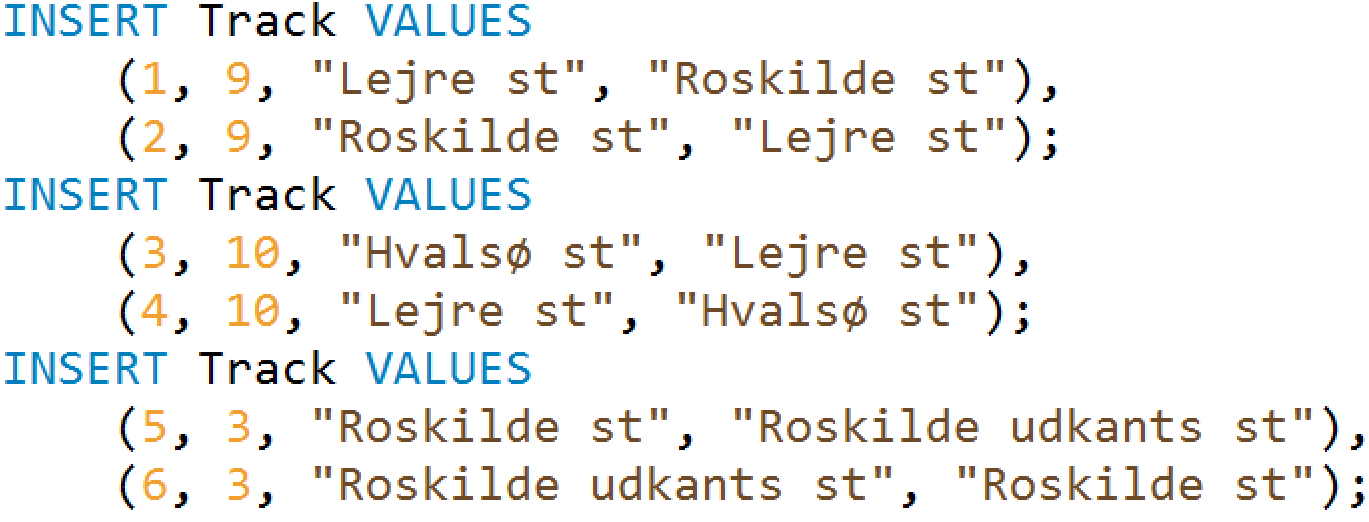
\includegraphics[width=1\textwidth]{img/INSERT_Statements_Track}
    \caption{SQL INSERT statements for Track}
\end{figure}

Finally, we can now insert routes that are composed of existing tracks.

\begin{figure}[ht!]
    \centering
    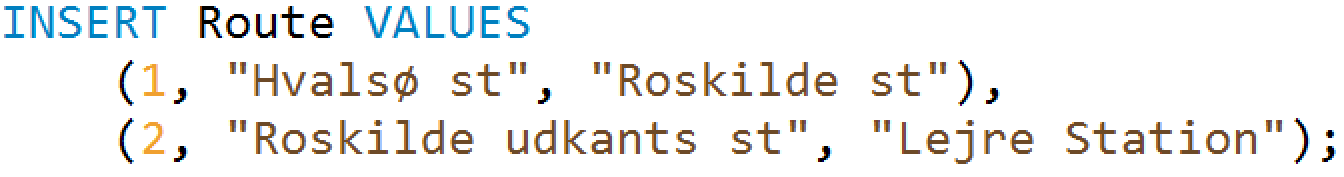
\includegraphics[width=.6\textwidth]{img/INSERT_Statements_Route}
    \caption{SQL INSERT statements for Route}
\end{figure}

When routes have been inserted it is necessary to have a relation containing 
which tracks each route is composed of. This is the \emph{RouteTracks} 
relation, which we will insert into now.

\begin{figure}[ht!]
    \centering
    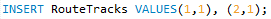
\includegraphics[width=.5\textwidth]{img/INSERT_Statements_RouteTracks}
    \caption{SQL INSERT statements for RouteTracks}
\end{figure}

We are now interested in having trains driving on these existing routes.

\begin{figure}[ht!]
    \centering
    
\includegraphics[width=.5\textwidth]{img/INSERT_Statements_Train}
    \caption{SQL INSERT statements for Train}
\end{figure}

However, a train does not have to be on a route. Say, it could be at the 
workshop, but it is still an existing train.

There is of course employees driving and controlling these trains, so lets 
insert some employees

\begin{figure}[ht!]
    \centering
    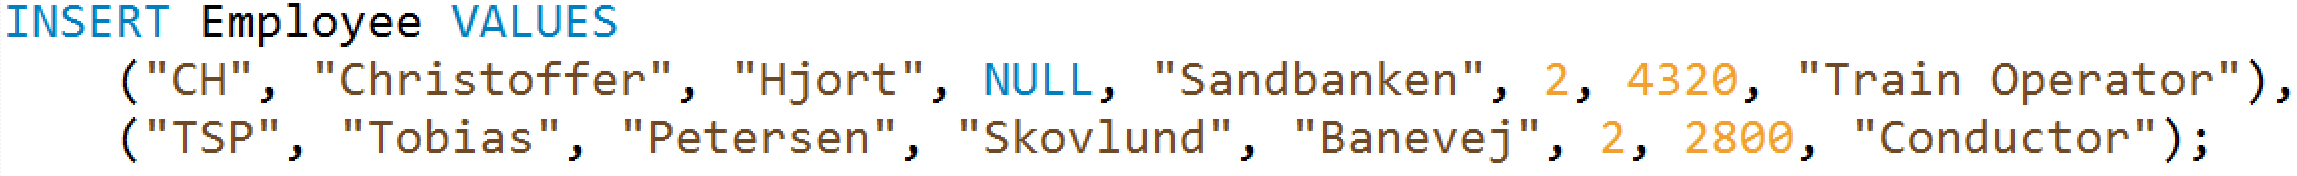
\includegraphics[width=1\textwidth]{img/INSERT_Statements_Employee}
    \caption{SQL INSERT statements for Employee}
\end{figure}

An employee can have a workshift on a train, which is stored as a tuple in the 
\emph{Shift} relation.

\begin{figure}[ht!]
    \centering
    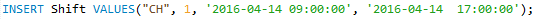
\includegraphics[width=.9\textwidth]{img/INSERT_Statements_Shift}
    \caption{SQL INSERT statements for Shift}
\end{figure}

When deleting tuples or dropping relations, the total participation of the 
relations comes into play again, just like when inserting into the schema.\\
In the \emph{Train Management} schema, the relations with total participation 
has been set to \emph{ON DELETE CASCADE}. So, if you were to delete a city 
which contained stations connected with tracks and routes, it would delete the 
routes, tracks and stations as well.\\

\begin{figure}[ht!]
    \centering
    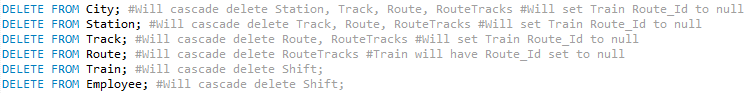
\includegraphics[width=1\textwidth]{img/DELETE_Statements}
    \caption{SQL DELETE statements}
\end{figure}

Not having the relations set to \emph{ON DELETE CASCADE}, the relations would 
have to be deleted in the correct order, starting from the bottom of the above 
figure.
Updates do not cascade, as the primary keys and foreign keys of relations 
should never need to be changed/updated. ID's should always stay the same, so 
``should'' city names and stations names. If a route were to have its start or 
stop station changed, we would simply insert a new route, rather than updating 
the old.
There are still other attributes that are useful to update though, as seen in 
the examples below.

\begin{figure}[ht!]
    \centering
    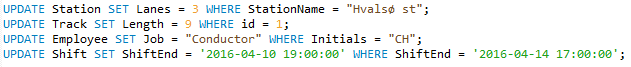
\includegraphics[width=1\textwidth]{img/UPDATE_Statements}
    \caption{SQL UPDATE statements}
\end{figure}

Some of the informations that should be retrieval according to the design, 
turned out to not be convenient to model directly, as for instance the length 
of a route. The entity \emph{Route} could have had an attribute with the length 
of the entire route, but this would be compromising the normalisations as the 
value should be calculated as the sum of lengths of all the tracks on the 
route. We therefore created the a view, that shows the length of all the 
tracks. The view, together with its implementation, can be seen in 
Figure~\ref{fig:length}.

\begin{figure}[h]
    \centering
    \begin{subfigure}[b]{0.45 \textwidth}
        \centering
        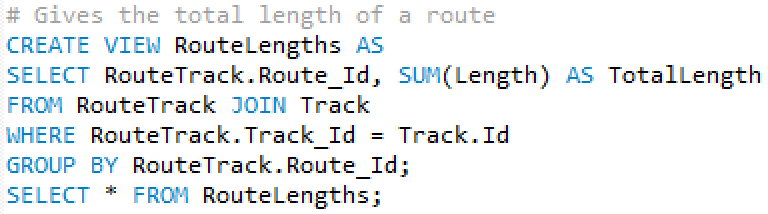
\includegraphics[width=\textwidth]{img/RouteLengths}
        \caption{Implementation of the view}
    \end{subfigure}
    \begin{subfigure}[b]{0.45 \textwidth}
        \centering
        PLACEHOLDER
%        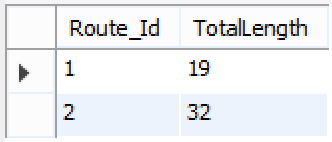
\includegraphics{img/RouteLengthsView}
        \caption{Selecting everything from the view}
    \end{subfigure}
    \caption{View for finding the lengths of all routes}
    \label{fig:length}
\end{figure}

Having implemented the first view we proceeded to implement views to get all 
the stations on a certain route. However, this turned out to be a fencepost 
problem, since we get the stations on the route, through the \emph{Track} 
entity. By selecting either the \emph{FromStation} or the \emph{ToStation} from 
all the tracks on the route, we would be missing either the first or the last 
station. We instead chose to select both and thus have a table of tracks 
(defined by pairs of stations), rather than stations. An example of this can be 
seen in Figure~\ref{fig:route}. Here the result is ordered by the attribute 
\emph{Number} which assures the tracks are listed in proper order (assuming of 
course that these numbers have been set properly).


\begin{figure}[h]
    \centering
    \begin{subfigure}[b]{0.45 \textwidth}
        \centering
        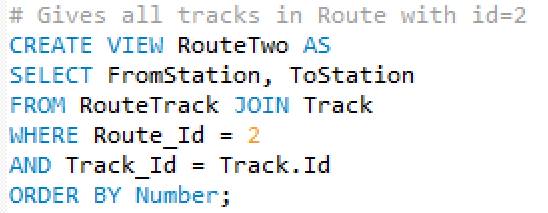
\includegraphics[width=\textwidth]{img/RouteTwo}
        \caption{Implementation of the view}
    \end{subfigure}
    \begin{subfigure}[b]{0.45 \textwidth}
        \centering
        PLACEHOLDER
        %        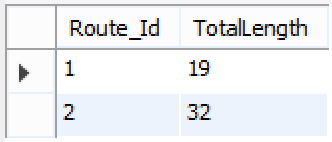
\includegraphics{img/RouteLengthsView}
        \caption{Selecting everything from the view}
    \end{subfigure}
    \caption{View of all tracks on route 2}
    \label{fig:route}
\end{figure}

\subsection{SQL Programming}
To control the data integrity and make insertion easier and less trivial or 
calculating attributes, a couple of functions, triggers, procedures, 
transactions and events have been programmed and implemented.

Each station has a specific capacity, that is amount of lanes. And, to make 
sure that no more tracks are connected to a station than there is capacity, a 
trigger has been implemented to prevent insertion.

\begin{figure}[ht!]
    \centering
    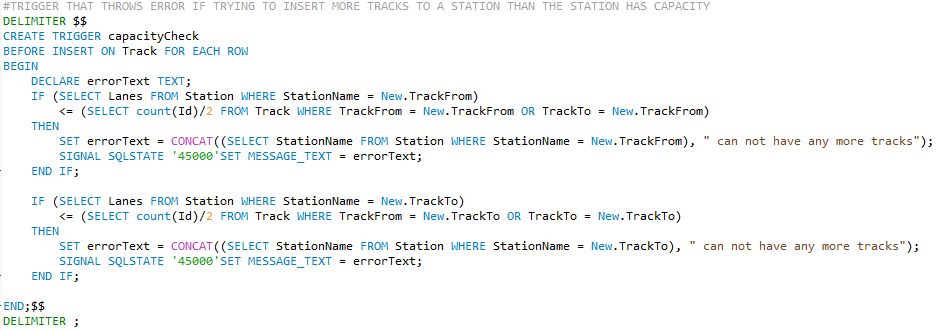
\includegraphics[width=1\textwidth]{img/SQL_TRIGGER}
    \caption{SQL Trigger}
\end{figure}

For example, if Station A has 2 lanes, which is equals to 4 tracks (For each 
lane there is 1 ingoing track and 1 outgoing), then the trigger would throw an 
error 1644, and prevent insertion of connecting a fifth track to Station A.

\begin{figure}[ht!]
    \centering
    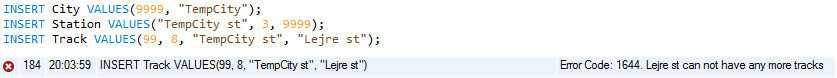
\includegraphics[width=1\textwidth]{img/SQL_TRIGGER_example}
    \caption{SQL Trigger example}
\end{figure}

Lejre st has 2 lanes and already had 4 tracks connected (2 tracks for each 
connected city), so trying to connect a fifth resulted in an error from the 
Trigger which triggers \emph{BEFORE INSERT}.

A couple of functions has also been implemented. These are primarily used to 
calculate dynamic attributes for the relations.
This is used calculating the length of a route

\begin{figure}[ht!]
    \centering
    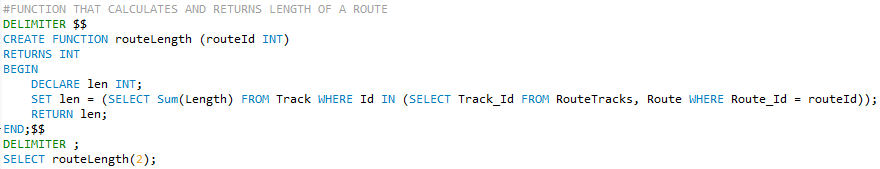
\includegraphics[width=1\textwidth]{img/SQL_FUNCTION_Length}
    \caption{SQL Function for Track Length}
\end{figure}

A function for calculating the age of a train.

\begin{figure}[ht!]
    \centering
    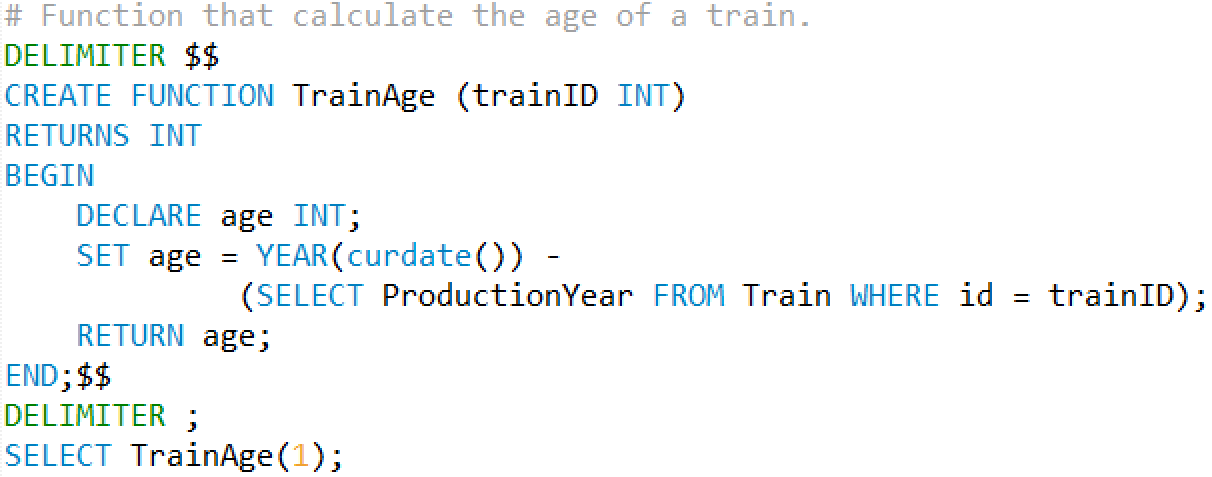
\includegraphics[width=1\textwidth]{img/SQL_FUNCTION_Age}
    \caption{SQL Function for Train Age}
\end{figure}

Next up is the implemented procedures. Some of the procedures only reads from 
the tables, while other procedures also performs data manipulation.

\begin{figure}[ht!]
    \centering
    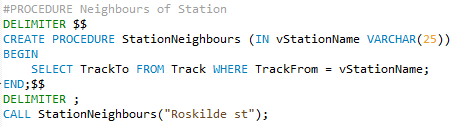
\includegraphics[width=1\textwidth]{img/SQL_PROCEDURE_Neighbours}
    \caption{SQL Procedure for finding Station neighbours}
\end{figure}

\begin{figure}[ht!]
    \centering
    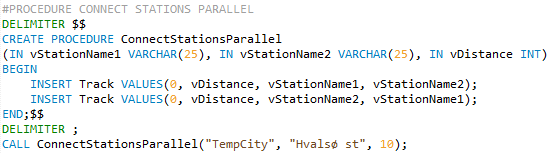
\includegraphics[width=1\textwidth]{img/SQL_PROCEDURE_ConnectParallel}
    \caption{SQL Procedure for connecting stations parallel both ways}
\end{figure}

The procedure inputs 0 to the ID's of the tracks, because our ID's 
automatically increments from the newest ID.

In this last procedure, a transaction has been included. This is to make sure, 
that the city and station do not get inserted unless it is possible to connect 
it to the targeted station.

\begin{figure}[ht!]
    \centering
    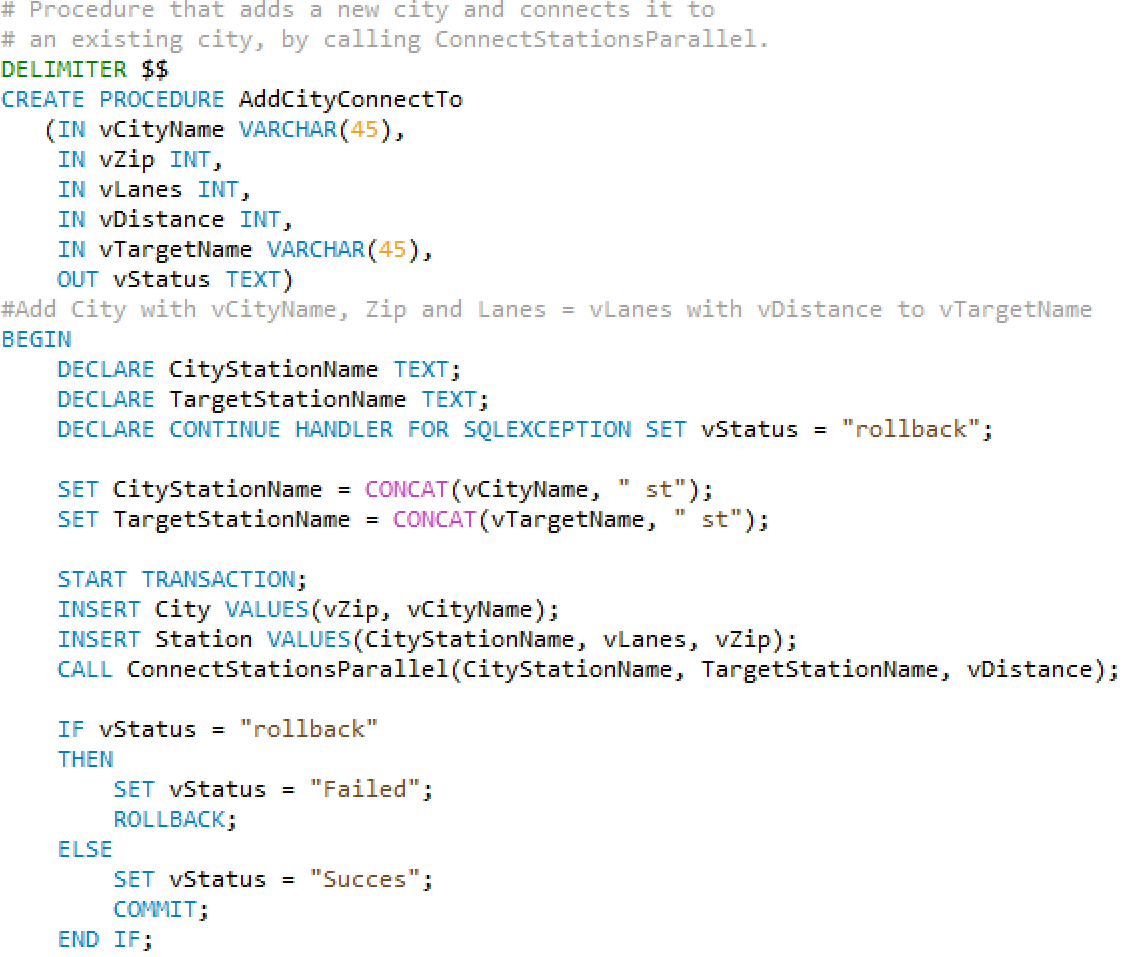
\includegraphics[width=1\textwidth]{img/SQL_PROCEDURE_AddCityConnect}
    \caption{SQL Procedure for connecting new city to target city}
\end{figure}

The procedure adds a new city to the database, creates the main station for the 
city, and connects it to the specified existing target city, with a specified 
distance, by adding tracks between them.

\begin{figure}[ht!]
    \centering
    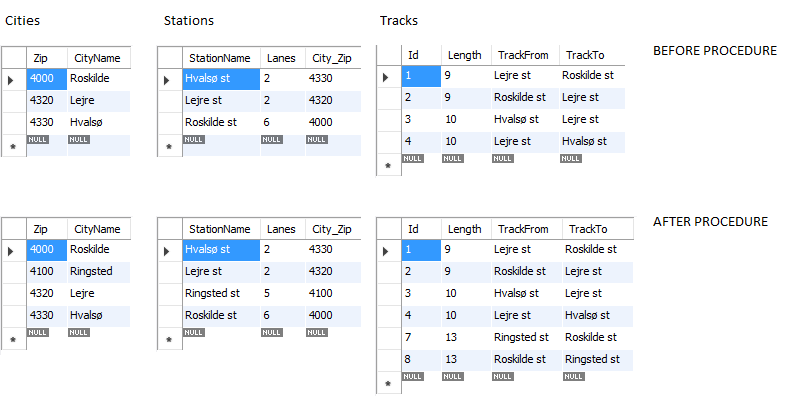
\includegraphics[width=1\textwidth]{img/SQL_PROCEDURE_AddCityConnect_example}
    \caption{Before and after the above procedure}
\end{figure}

The only event, is really not a required functionality, as our \emph{Train 
Management} schema really has no need of events in its current state. 

\begin{figure}[ht!]
    \centering
    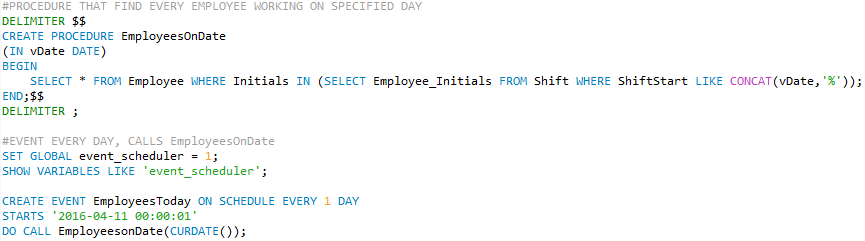
\includegraphics[width=1\textwidth]{img/SQL_EVENT}
    \caption{SQL Event for finding todays employees}
\end{figure}

This event tells who is at work everyday.
The implemented event, is more for general managing, as it is nice to know for 
each day of the week what employees are at work.

    \section{Conclusion}
% Tobias

% Discussion paragraphs first (if any)

% Comment on final result
The goal of the project was to generate a functioning database train 
management. We did this by first designing the database as en Entity Relation 
diagram. Once the diagram was finished it was translated into the MySQL EER 
diagram. However, at this point we realised flaws in the initial design, and an 
iterative process thereby began. One entity or relation was translated possibly 
redesigned translated again. Only once we were satisfied, we moved on to the 
next relation/entity. This gave a nice workflow as each aspect of the database 
was considered in turn.

% Does the implementation follow the design (YES - generated from "sketch")
% Where does it not? Why?
After the design (ER diagram) had been translated to the EER diagram, the 
database could be forward engineered. This had the huge advantage that 
implementation automatically becomes very much like the design, assuming the 
translation did not change too much. By very little effort the ``sketch'' of a 
database was made into an actual database, at which point we could start 
programming functionality.

% Comments on work -process, -flow, and possibly -distribution
% Mentioned briefly above

% Future expansions?
If we were to further develop the database, there are several aspects that 
could be improved. First of all we have only dealt with the actual database. 
There exists no presentation layer. A nice extension would therefore be to 
build a front end for the database. The database also suffers from being a 
local instance. For the database to actually be used to manage trains, it would 
need to be accessible for many people possibly at various locations. It would 
therefore need to be accessible online. However, staying with database 
improvements a natural progression of the project would be to look into 
timeslots. The trains arrive and leave stations at specific times on specific 
days. Modelling this would be a natural extension to our database. 

    
    \appendix
    \section{Forward Engineered Database}

Content of the file TrainManagement.sql:

\lstinputlisting[ ]
{../TrainManagement.sql}

	%\include{SQL_data_manipulation}
    %\include{SQL_programming}
    
\end{document}
